\section{Dataset and Exploratory Analysis}
\subsection{Data and Sparse Storage}
MovieLens 32M contains 32,000,204 ratings from 200,948 users across 87,585 catalog movies \citep{movielens32m,harper2015}. Ratings range from 0.5 to 5 in half-star steps. The release selects users with at least 20 ratings. All observations and catalog movies are retained.

\begin{table}[H]
\caption{Complete dataset and seeded 80/20 split.}
\label{tab:data}\centering\small
\begin{tabular*}{\linewidth}{@{\extracolsep{\fill}}lr}\toprule
Quantity & Count\\\midrule
All ratings & 32,000,204\\
Users & 200,948\\
Catalog movies & 87,585\\
Training ratings & 25,601,250\\
Test ratings & 6,398,954\\
Movies without training ratings & 7,319\\\bottomrule
\end{tabular*}
\end{table}

The observed matrix is 0.18\% dense; a dense float32 representation would need about 65.6 GiB. IDs map to contiguous indices. Chunked loading writes indices, ratings, and split membership to disk-backed arrays. Training entries are indexed in compressed sparse rows by both user and movie. Missing entries are unobserved preferences, not zero ratings.

The catalog includes 3,153 movies without any ratings and 7,319 without training ratings. Every user has training data, with a minimum of eight observations.

\subsection{Distributions}
Four stars is the most frequent rating (Figure~\ref{fig:ratings}). Activity and movie support have long tails (Figure~\ref{fig:degree}), reflecting uneven feedback. Discrete frequency counts produce the horizontal tail bands; the plot alone does not establish a power law.

\begin{figure}[H]
\centering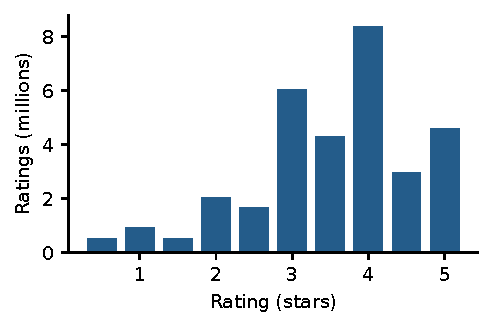
\includegraphics[width=\columnwidth]{rating_distribution.pdf}
\caption{Rating distribution over all 32,000,204 observations.}
\label{fig:ratings}\end{figure}
\begin{figure}[H]
\centering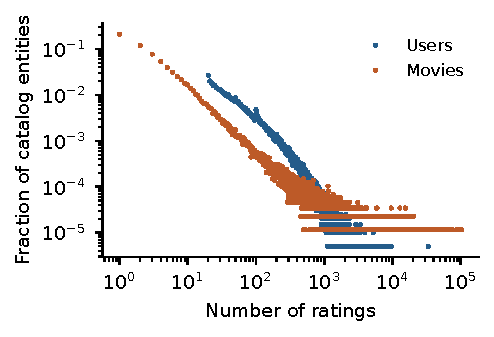
\includegraphics[width=\columnwidth]{degree_distribution.pdf}
\caption{User and movie degrees. Zero-degree movies remain in the denominator but cannot appear on the log axis.}
\label{fig:degree}\end{figure}
